\documentclass[12pt]{article}
\usepackage{graphicx} % Required for inserting images



\begin{document}


\section*{Digital assignment}
\subsection*{Roll number : ee23btech11220}


\section{\textbf{Problem 11.9.5.22}}
$$2\times4+4\times6+6\times8\cdots+n\,terms$$ 


Find the 20th term in this series.\\

\textbf{Given,}
series is of the form
\begin{equation}
\sum_{r=1}^{r=n} 2*r*2*(r+1)
\end{equation}
\begin{equation}
\sum_{r=1}^{r=n} 4*r*(r+1)
\end{equation}
So $20^{th}$ term of this series is obtained by substituting r=20 in\\ $4*r*(r+1)$
= 4*20*21
= 80*21
=1680

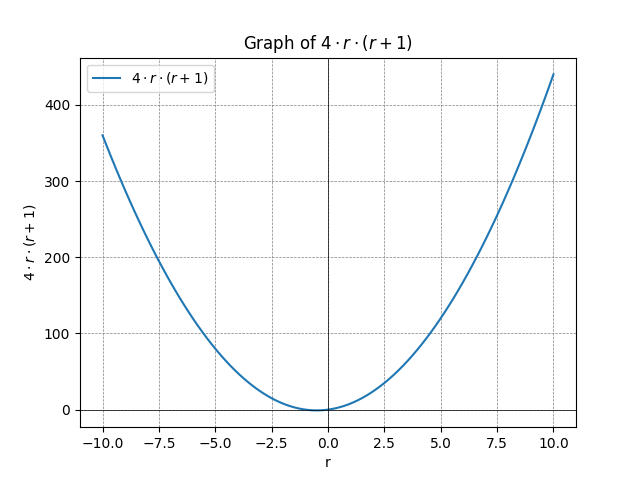
\includegraphics[scale=0.8]{assignments/digital2/graphs/graph2.png}
\end{document}
